\section{Dataset clusters comparison}

		\begin{figure*}[ht!]
			\centering
			\subfloat[Zernike coefficients]{%
				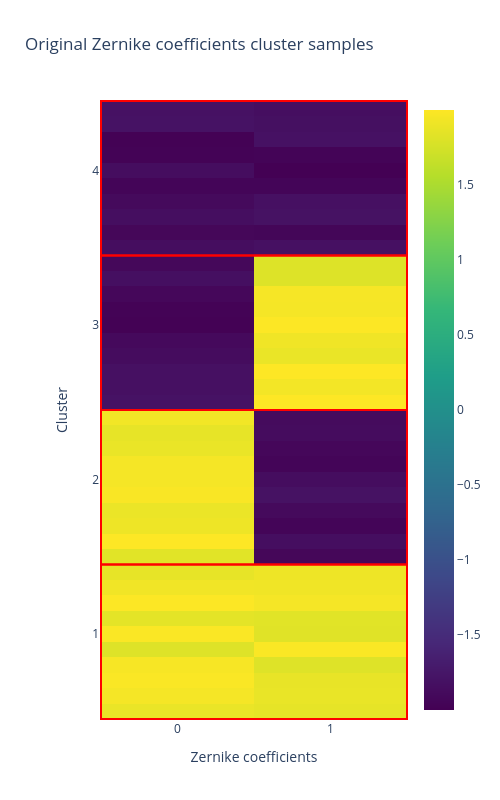
\includegraphics[width=0.22\textwidth]{mdid-zernikecoefficientsoriginalgridclusters.png}}
			\hspace{\fill}
			\subfloat[LP coefficients]{%
				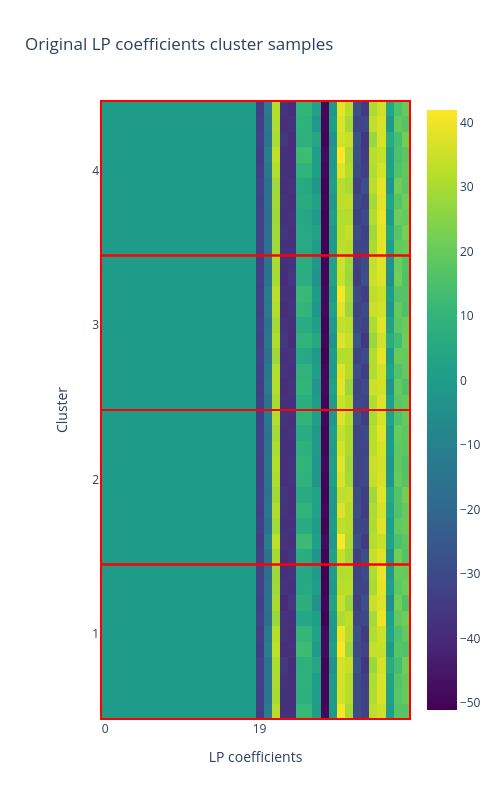
\includegraphics[width=0.22\textwidth]{mdid-lpcoefficientsoriginalgridclusters.png}}
			\hspace{\fill}
			\subfloat[Output fluxes]{%
				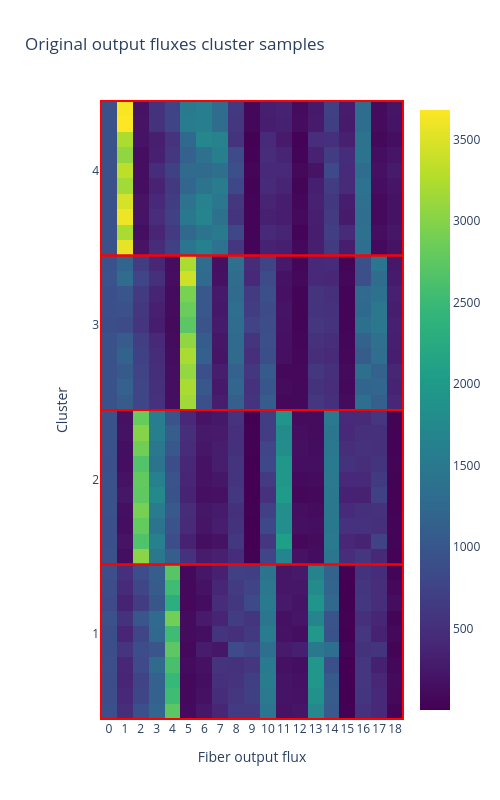
\includegraphics[width=0.22\textwidth]{mdid-outputfluxesoriginalgridclusters.png}}
			\hspace{\fill}
			\subfloat[PCA PSF Intensities]{%
				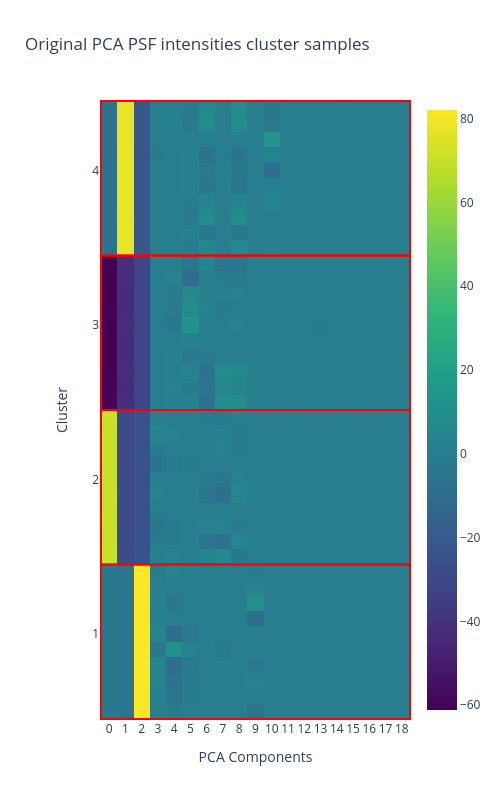
\includegraphics[width=0.22\textwidth]{mdid-pcaintensitiesoriginalgridclusters.png}}
			\hspace{\fill}
			\caption{Original clusters from the datasets}
		\end{figure*}
		\FloatBarrier
		
		\begin{figure*}[ht!]
			\centering
			\subfloat[Zernike coefficients]{%
				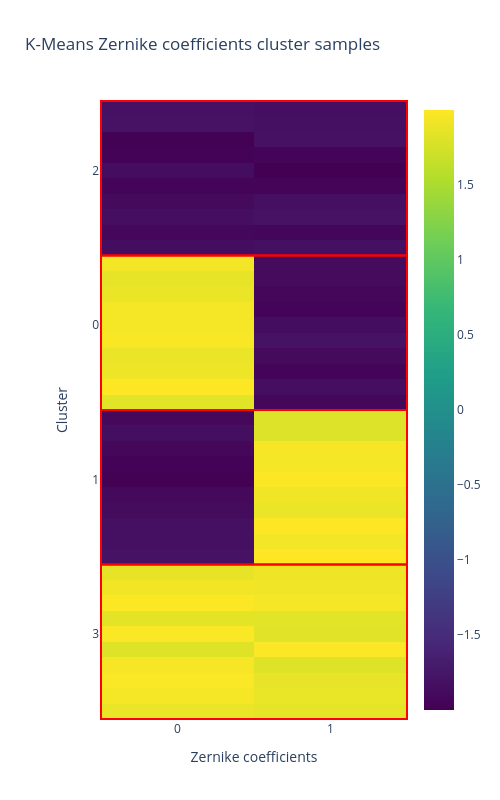
\includegraphics[width=0.22\textwidth]{mdid-zernikecoefficientsK-Meansgridclusters.png}}
			\hspace{\fill}
			\subfloat[LP coefficients]{%
				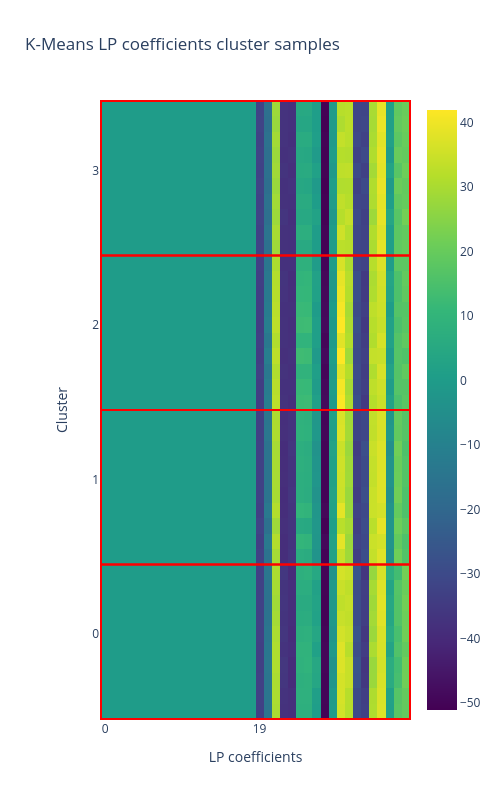
\includegraphics[width=0.22\textwidth]{mdid-lpcoefficientsK-Meansgridclusters.png}}
			\hspace{\fill}
			\subfloat[Output fluxes]{%
				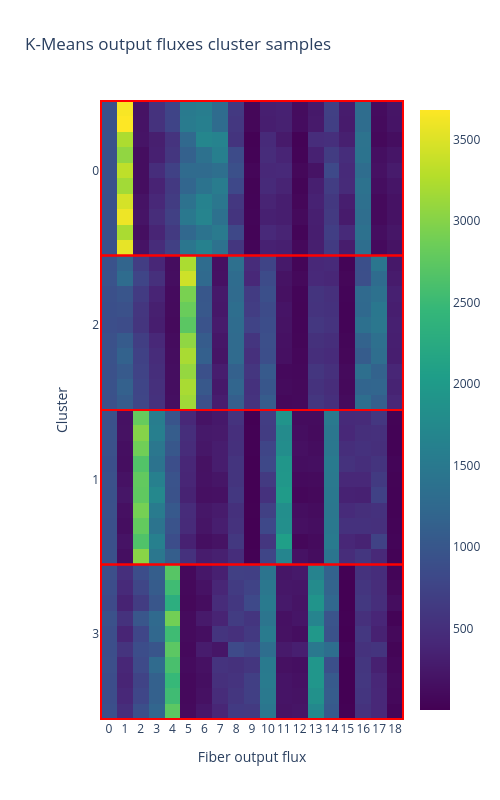
\includegraphics[width=0.22\textwidth]{mdid-outputfluxesK-Meansgridclusters.png}}
			\hspace{\fill}
			\subfloat[PCA PSF Intensities]{%
				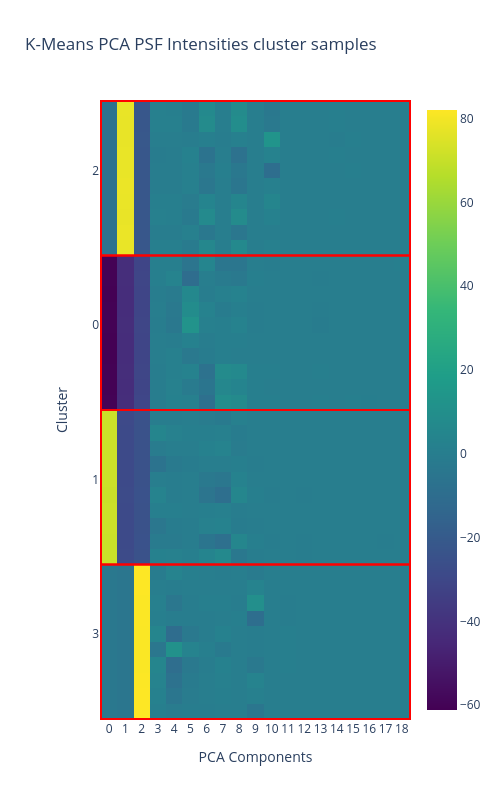
\includegraphics[width=0.22\textwidth]{mdid-pcaintensitiesK-Meansgridclusters.png}}
			\hspace{\fill}
			\caption{K-Means clusters from the datasets}
		\end{figure*}
		\FloatBarrier
		
		\begin{figure*}[ht!]
			\centering
			\subfloat[Zernike coefficients]{%
				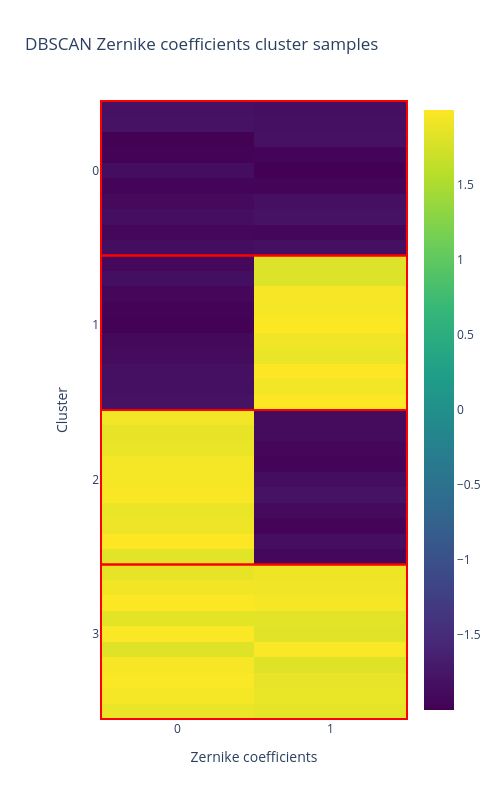
\includegraphics[width=0.22\textwidth]{mdid-zernikecoefficientsDBSCANgridclusters.png}}
			\hspace{\fill}
			\subfloat[LP coefficients]{%
				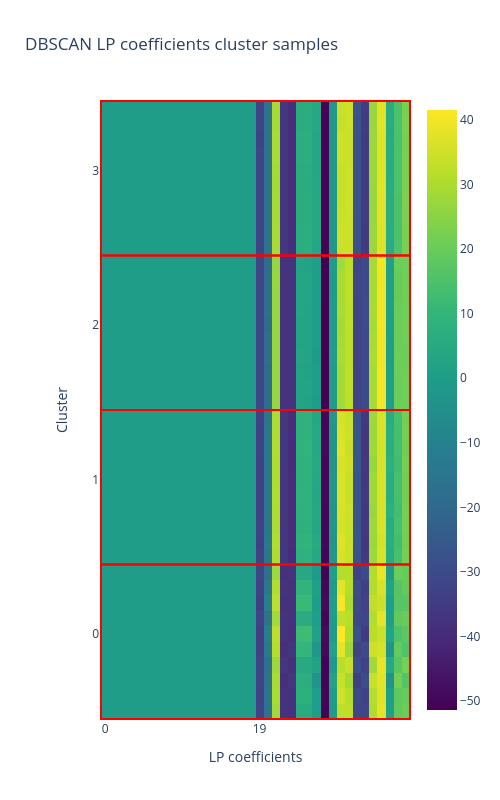
\includegraphics[width=0.22\textwidth]{mdid-lpcoefficientsDBSCANgridclusters.png}}
			\hspace{\fill}
			\subfloat[Output fluxes]{%
				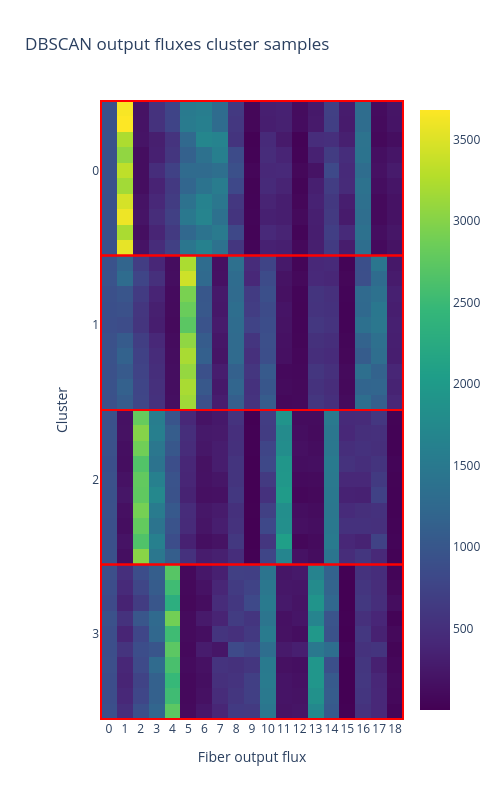
\includegraphics[width=0.22\textwidth]{mdid-outputfluxesDBSCANgridclusters.png}}
			\hspace{\fill}
			\subfloat[PCA PSF Intensities]{%
				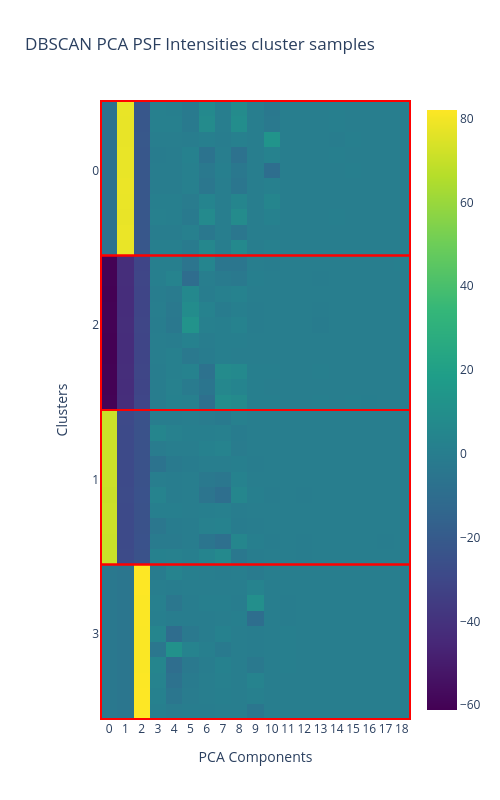
\includegraphics[width=0.22\textwidth]{mdid-pcaintensitiesDBSCANgridclusters.png}}
			\hspace{\fill}
			\caption{DBSCAN clusters from the datasets}
		\end{figure*}
		\FloatBarrier
		
		\begin{figure*}[ht!]
			\centering
			\subfloat[Zernike coefficients]{%
				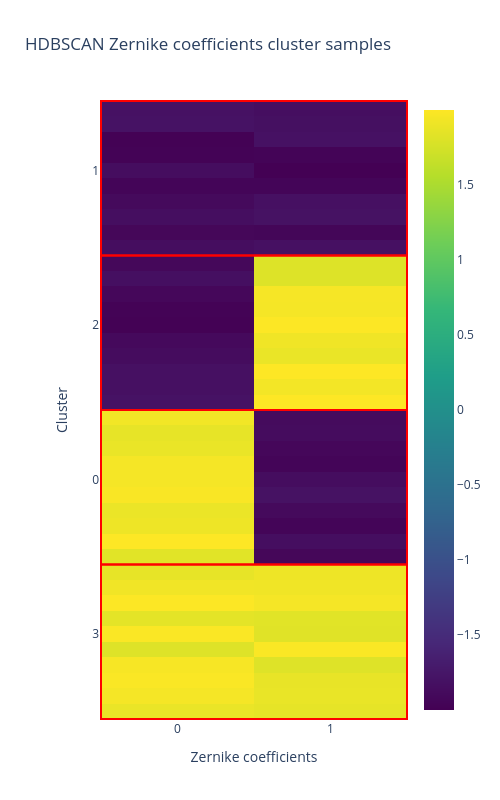
\includegraphics[width=0.22\textwidth]{mdid-zernikecoefficientsHDBSCANgridclusters.png}}
			\hspace{\fill}
			\subfloat[LP coefficients]{%
				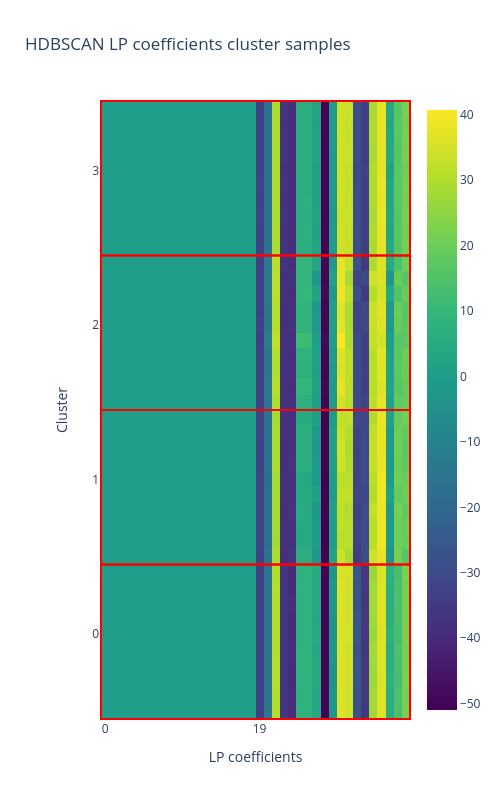
\includegraphics[width=0.22\textwidth]{mdid-lpcoefficientsHDBSCANgridclusters.png}}
			\hspace{\fill}
			\subfloat[Output fluxes]{%
				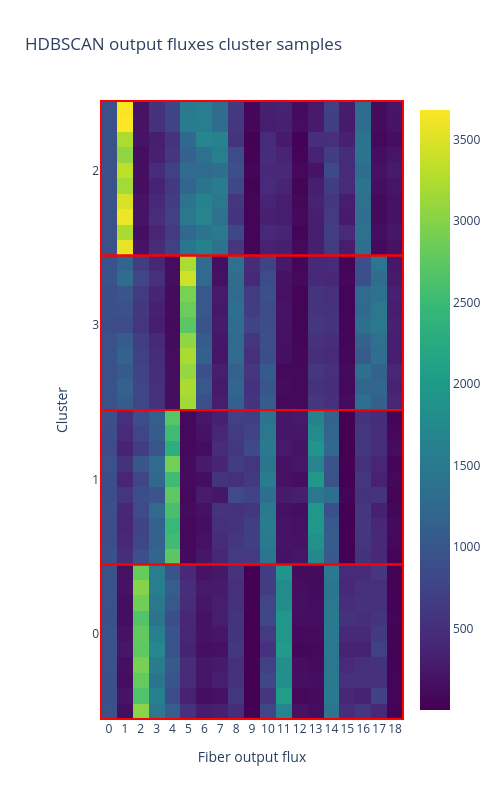
\includegraphics[width=0.22\textwidth]{mdid-outputfluxesHDBSCANgridclusters.png}}
			\hspace{\fill}
			\subfloat[PCA PSF Intensities]{%
				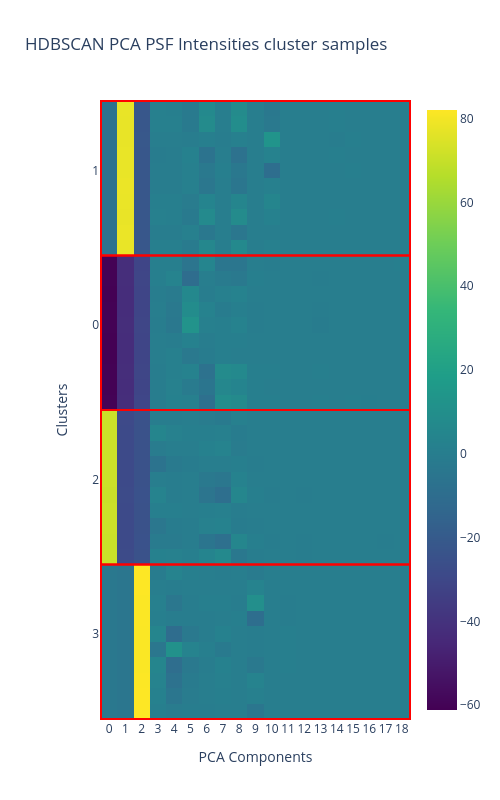
\includegraphics[width=0.22\textwidth]{mdid-pcaintensitiesHDBSCANgridclusters.png}}
			\hspace{\fill}
			\caption{HDBSCAN clusters from the datasets}
		\end{figure*}
		\FloatBarrier
		
		\begin{figure*}[ht!]
			\centering
			\subfloat[Zernike coefficients]{%
				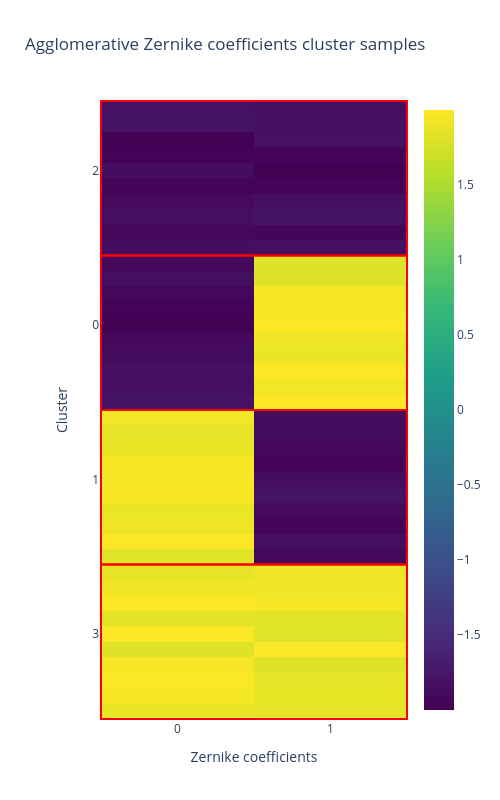
\includegraphics[width=0.22\textwidth]{mdid-zernikecoefficientsAgglomerativegridclusters.png}}
			\hspace{\fill}
			\subfloat[LP coefficients]{%
				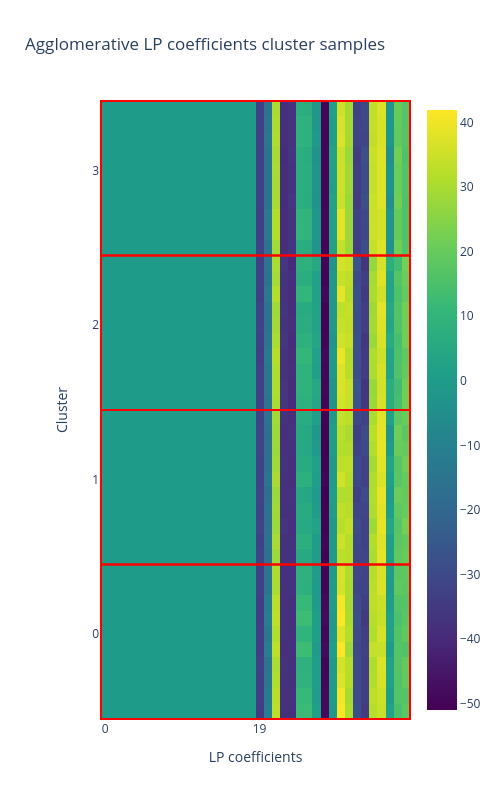
\includegraphics[width=0.22\textwidth]{mdid-lpcoefficientsAgglomerativegridclusters.png}}
			\hspace{\fill}
			\subfloat[Output fluxes]{%
				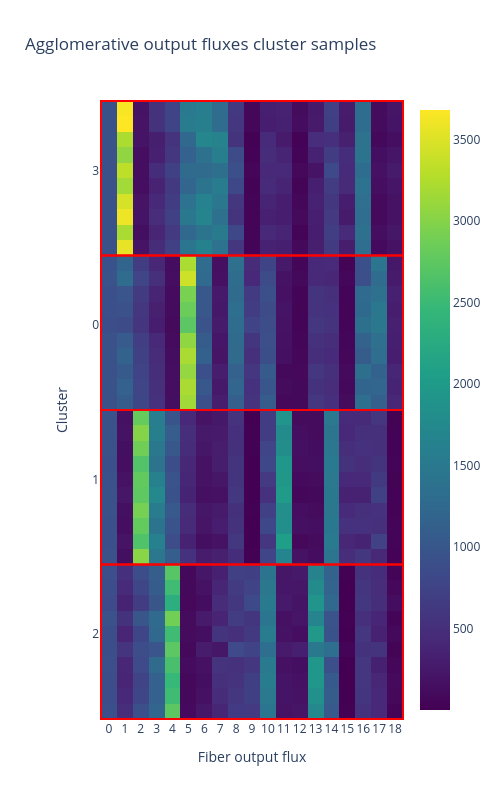
\includegraphics[width=0.22\textwidth]{mdid-outputfluxesAgglomerativegridclusters.png}}
			\hspace{\fill}
			\subfloat[PCA PSF Intensities]{%
				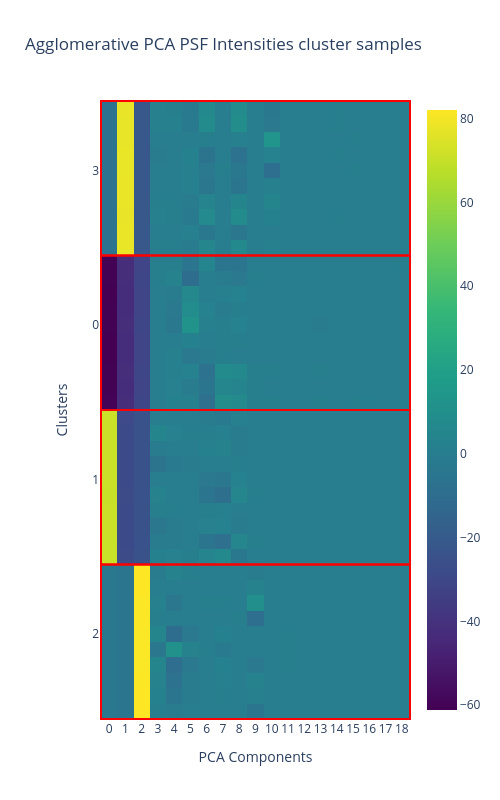
\includegraphics[width=0.22\textwidth]{mdid-pcaintensitiesAgglomerativegridclusters.png}}
			\hspace{\fill}
			\caption{Agglomerative clusters from the datasets}
		\end{figure*}
		\FloatBarrier